\chapter{MongoDb}

\section{Caratteristiche}

MongoDb e' uno dei piu' diffusi database non relazionali orientato ai documenti, di tipo NoSQL,  utilizza documenti in un formato JSON al posto delle tipiche tabelle 
dei sistemi relazionali. Piu' precisamente MongoDb utilizza i BSON ossia JSON binari per rappresentare strutture dati semplici e array associativi (oggetti in MongoDb),
un BSON contiene una lista ordinata di elementi appartenenti ai seguenti tipi:

\begin{itemize}{}{}
    \item stringhe
    \item interi (32 o 64 bit)
    \item double (numeri a virgola mobile a 64 bit, standard IEEE 754)
    \item date (numeri interi in millisecondi dal'epoca Unix come riferimento, 1º gennaio 1970)
    \item byte array (dati binari)
    \item booleani (true e false)
    \item NULL
    \item oggetto BSON
    \item array BSON
    \item espressioni regolari
    \item codice JavaScript
\end{itemize}

\section{Organizzazione dei dati}

\subsection{Creazione collezioni}

Per poter originare i set di dati sui quali lavoriamo siamo partiti da 2 enormi file JSON generati al paragrafo ??????????? //TODO riguarda qua //
contenenti POST (A) e COMMENTI(B). Il paramentro \$out posto dopo la query ha creato una collezione a tuttli gli effetti sulla quale poter eseguire le query
all'interno della rete del container.

\subsubsection{Referencing}

Il referencing di A in B si ottiene facilmente proiettando gli attributi della collezione B, dato che contiene al suo interno la foreign Key di A.

\subsubsection{Referencing di A in B}

\begin{verbatim}
db.B.aggregate([
  {
    $project: {
      "_id" : "$BK",
      "BK" : "$BK",
      "AK" : "$FAK",
      "B1" : "$B1",   
      "B2" : "$B2",
      "B3" : "$B3",
      "B4" : "$B4",
      "B5" : "$B5",
      "B6" : "$B6",
      "B7" : "$B7"
    }
  },{
  $out : "referencing_A_in_B"
}
])
\end{verbatim}

\fvset{gobble=2}
\begin{Verbatim}[frame=single,framesep=2mm,label= Referencing di A in B,labelposition=all]
{
  "_id": 21748,
  "BK": 21748,
  "AK": 70394,
  "B1": 85337,
  "B2": 255,
  "B3": 6,
  "B4": 85337,
  "B5": 255,
  "B6": 6,
  "B7": "Lorem ipsum dolor sit amet, consectetur adipiscing elit. 
    Fusce lacinia eget arcu et maximus. Ut tempus est sit amet 
    tortor commodo, sit amet facilisis mi rhoncus. Donec et elit
    venenatis, consequat tellus eu, tristique orci. Duis 
    tristique sem ut nulla ullamcorper, a porta risus efficitur.
    Cras sed neque et nisl tincidunt vestibulum. Phasellus 
    tristique tempor facilisis. Sed facilisis lectus eros, sed 
    aliquet lacus elementum sed. Integer vel dictum mi. 
    Maecenas pharetra tempus eros, efficitur mattis erat cursus
    in. Nulla sit amet quam velit. Nullam tempus dictum lacus
    id porttitor. Vestibulum facilisis pulvinar fermentum.
    Ut elementum maximus feugiat. In at mollis leo, eu 
    facilisis magna. Vestibulum sed nisi ultricies, tincidunt
    enim ac, fringilla ex. Phasellus pharetra mollis nisi
    a fermentum. In nec faucibus nulla, eget molestie magna.
    Vivamus in gravida ex. Aenean scelerisque gravida 
    ipsum, nec congue enim posuere sit amet. Donec vitae felis
    id sem congue blandit eget non justo quis."
}
\end{Verbatim}

Il referencing di B in A invece richiede un join, un' operazione piu' onerosa per la quale ho dovuto passare il parametro allowDiskUse=true per poter utilizzare
a pieno la memoria della macchina e quindi eseguire il join trovando di fatto le chiavi e aggiungendole all'array B che arrivera' a contenere 10 chivi BK per ogni 
AK dato che il rapporto e' di 1:10. 

\subsubsection{Referencing di B in A}

\begin{verbatim}
    
db.B.aggregate(
[
   {
      $group: {
        _id: {"AK" : "$FAK"}, "BK": {$addToSet : "$BK"}
      }
    },
    {
      $lookup: {
        from: 'Ap',
        localField: '_id.AK',
        foreignField: 'AK',
        as: 'AK'
      }
    },{
      $project : {"_id" : 0,"BK.FAK" : 0}
    },{
    $unwind: {
      path: "$AK",
    }},{
      $project : {
      "_id" : "$AK.AK",
      "AK" : "$AK.AK",
      "A1" : "$AK.A1", 
      "A2" : "$AK.A2", 
      "A3" : "$AK.A3", 
      "A4" : "$AK.A4",
      "A5" : "$AK.A5",
      "A6" : "$AK.A6",
      "A7" : "$AK.A7",
       "B" : "$BK"} 
    },{
      $out : "referencing_B_in_A"
    }
  ],{allowDiskUse:true}
)
\end{verbatim}

\fvset{gobble=2}
\begin{Verbatim}[frame=single,framesep=2mm,label= Referencing di B in A,labelposition=all]
{
  "_id": 8518,
  "AK": 8518,
  "A1": 6773,
  "A2": 253,
  "A3": 4,
  "A4": 6773,
  "A5": 253,
  "A6": 4,
  "A7": "Lorem ipsum dolor sit amet, consectetur adipiscing elit. 
    Fusce lacinia eget arcu et maximus. Ut tempus est sit amet 
    tortor commodo, sit amet facilisis mi rhoncus. Donec et elit
    venenatis, consequat tellus eu, tristique orci. Duis 
    tristique sem ut nulla ullamcorper, a porta risus efficitur.
    Cras sed neque et nisl tincidunt vestibulum. Phasellus 
    tristique tempor facilisis. Sed facilisis lectus eros, sed 
    aliquet lacus elementum sed. Integer vel dictum mi. 
    Maecenas pharetra tempus eros, efficitur mattis erat cursus
    in. Nulla sit amet quam velit. Nullam tempus dictum lacus
    id porttitor. Vestibulum facilisis pulvinar fermentum.
    Ut elementum maximus feugiat. In at mollis leo, eu 
    facilisis magna. Vestibulum sed nisi ultricies, tincidunt
    enim ac, fringilla ex. Phasellus pharetra mollis nisi
    a fermentum. In nec faucibus nulla, eget molestie magna.
    Vivamus in gravida ex. Aenean scelerisque gravida 
    ipsum, nec congue enim posuere sit amet. Donec vitae felis
    id sem congue blandit eget non justo quis.",
  "B": [
    182143,
    450648,
    120258,
    151670,
    314940,
    281717,
    335311,
    802016,
    313524,
    537
  ]
}
\end{Verbatim}

\subsubsection{Embedding}
Per l'embedding di documenti ho dovuto sempre eseguire dei join ma e' stato fondamentale poter aggiungere un intero documento all'interno di un'array tramite il parametro
\verb|$$ROOT| che ha permesso un operazione molto piu'veloce e compatta.

\subsubsection{Embedding di A in B}
 

\begin{verbatim}
db.B.aggregate(
  [
    {
      $lookup: {
        from: 'A',
        localField: 'FAK',
        foreignField: 'AK',
        as: 'A'
      }
    }
   ,{
     $project: {
       "FAK" : 0,
       "_id" : 0,
       "A._id" : 0
     }
   }
  ,{
    $project : {
      "_id" : "$BK",
      "B1" : 1,
      "B2" : 1,
      "B3" : 1,
      "B4" : 1,
      "B5" : 1,
      "B6" : 1,
      "B7" : 1,
      "A" : 1
    }
  }
  ,{
     $out : "embedding_A_in_B"
   }
  ]
)    
\end{verbatim}


\fvset{gobble=2}
\begin{Verbatim}[frame=single,framesep=2mm,label= Embedding di B in A,labelposition=all]
{
  "_id": 963593,
  "B1": 77221,
  "B2": 86,
  "B3": 1,
  "B4": 77221,
  "B5": 86,
  "B6": 1,
  "B7": [ ..... ],
  "A": [
    {
      "AK": 70394,
      "A1": 7960,
      "A2": 269,
      "A3": 8,
      "A4": 7960,
      "A5": 269,
      "A6": 8,
      "A7": [ ..... ]
    }
  ]
}
\end{Verbatim}

\subsubsection{Embedding di B in A}

\begin{verbatim}
    db.B.aggregate(
  [
   {
      $group: {
        _id: {"AK" : "$FAK"}, "BK": {$addToSet : "$$ROOT"}
      }
    },
    {
      $lookup: {
        from: 'A',
        localField: '_id.AK',
        foreignField: 'AK',
        as: 'AK'
      }
    },{
      $project : {"_id" : 0,"BK.FAK" : 0}
    },{
    $unwind: {
      path: "$AK",
    }},{
      $project : {
        "_id" : "$AK.AK",
        "AK" : "$AK.AK", 
        "A1" : "$AK.A1", 
        "A2" : "$AK.A2", 
        "A3" : "$AK.A3", 
        "A4" : "$AK.A4",
        "A5" : "$AK.A5",
        "A6" : "$AK.A6",
        "A7" : "$AK.A7",
        "B" : "$BK"} 
    },{
        $project : { "A._id" : 0, "B._id" : 0}
    },{
        $out : "embedding_B_in_A"
   }
  ],{allowDiskUse:true}
)
\end{verbatim}

\fvset{gobble=2}
\begin{Verbatim}[frame=single,framesep=2mm,label= Embedding di B in A,labelposition=all]
{
  "_id": 48,
  "AK": 48,
  "A1": 691,
  "A2": 154,
  "A3": 0,
  "A4": 691,
  "A5": 154,
  "A6": 0,
  "A7": [ ..... ],
  "B": [
    {
      "BK": 844575,
      "B1": 94813,
      "B2": 140,
      "B3": 2,
      "B4": 94813,
      "B5": 140,
      "B6": 2,
      "B7": [ ..... ]
    },
    {
      "BK": 115006,
      "B1": 36,
      "B2": 483,
      "B3": 8,
      "B4": 36,
      "B5": 483,
      "B6": 8,
      "B7": [ ..... ]
    },
    .
    .
    .
    .
    {
      "BK": 834226,
      "B1": 77768,
      "B2": 707,
      "B3": 6,
      "B4": 77768,
      "B5": 707,
      "B6": 6,
      "B7": [ ..... ]
    }
  ]
}
\end{Verbatim}
\subsection{Indici}

Gli indici per gli attributi sono stati creati attraverso uno script in JS che viene eseguito durante la creazione del container.

MongoDB utilizza, se non esplicitamente indicato, come strutture dati per gli indici dei B-tree. Dato che abbiamo scelto di adoperare l'embedding di interi documenti sono stati 
indicizzati anche gli attributi dei documenti "innestati" sui quali saranno esegeuite delle query, anche sulle foreign del referencing sono stati costruiti indici.

\begin{center}
  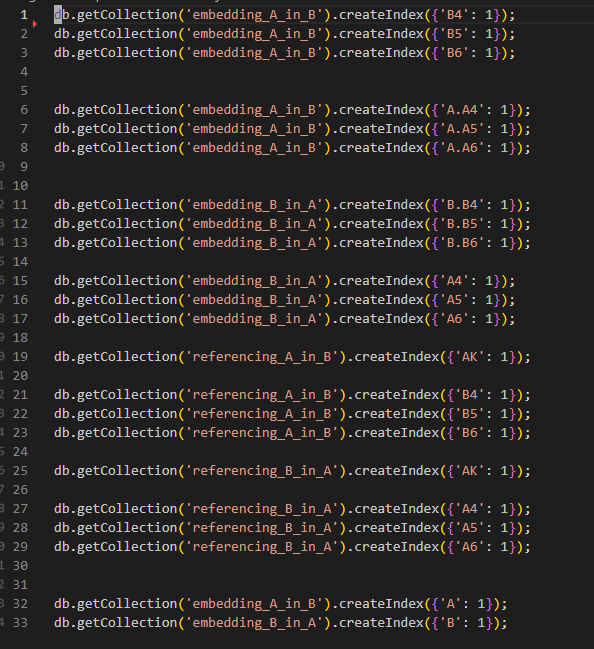
\includegraphics{../code/makeIndexes.png}
\end{center}

\begin{lstlisting}[caption=making indexes, style=customJs]
// indexes
db.getCollection('embedding_A_in_B').createIndex({'B4': 1});
db.getCollection('embedding_A_in_B').createIndex({'B5': 1});
db.getCollection('embedding_A_in_B').createIndex({'B6': 1});

// nested indexes
db.getCollection('embedding_A_in_B').createIndex({'A.A4': 1});
db.getCollection('embedding_A_in_B').createIndex({'A.A5': 1});
db.getCollection('embedding_A_in_B').createIndex({'A.A6': 1});

// indexes
db.getCollection('embedding_B_in_A').createIndex({'A4': 1});
db.getCollection('embedding_B_in_A').createIndex({'A5': 1});
db.getCollection('embedding_B_in_A').createIndex({'A6': 1});

// nested indexes
db.getCollection('embedding_B_in_A').createIndex({'B.B4': 1});
db.getCollection('embedding_B_in_A').createIndex({'B.B5': 1});
db.getCollection('embedding_B_in_A').createIndex({'B.B6': 1});

//FK
db.getCollection('referencing_A_in_B').createIndex({'AK': 1});               

// indexes
db.getCollection('referencing_A_in_B').createIndex({'B4': 1});
db.getCollection('referencing_A_in_B').createIndex({'B5': 1});
db.getCollection('referencing_A_in_B').createIndex({'B6': 1});

//FK
db.getCollection('referencing_B_in_A').createIndex({'AK': 1});               

// indexes
db.getCollection('referencing_B_in_A').createIndex({'A4': 1});
db.getCollection('referencing_B_in_A').createIndex({'A5': 1});
db.getCollection('referencing_B_in_A').createIndex({'A6': 1});

// array indexes
db.getCollection('embedding_A_in_B').createIndex({'A': 1});
db.getCollection('embedding_B_in_A').createIndex({'B': 1});
\end{lstlisting}

% \lstinputlisting[caption=making indexes, style=customJs]
